\chapter{État de l’art}

\section{Le dérèglement climatique}

Nous pouvons faire l’analogie avec une application logicielle. Une règle courante est d’éviter
l’optimisation prématurée, c’est à dire de ne pas optimiser tant que le besoin ne s’en fait pas
ressentir. Nous risquerions de dépenser du temps et de l'énergie dans quelques chose qui
peut-être ne fonctionne pas comme nous le voudrions.
Dans un premier temps, il faut faire en sorte que le système fonctionne correctement.
On peut préférer la quantité face à la qualité. On ne cherche à optimiser cette méthode
qu’ensuite, lorsque les ressources commencent à ne plus suffire ou qu’un besoin de remise
à l’échelle se fait sentir.

Aujourd'hui nous sommes en mesure de produire suffisamment d’énergie pour répondre aux
besoin de la population. Mais le contexte environnementale nous impose désormais d’optimiser
nos méthodes : épuisement des énergies fossiles, réchauffement climatique, augmentation de la
population.

\section{Augmentation des besoins en énergie}

L'énergie apporte l'augmentation de la consommation d'énergie, comme le montre la figure
\ref{fig:capita_energy}, chaque personne consomme plus d'énergie qu'un habitant
du début des années 1800.

\begin{SCfigure}[][h]
  \centering
  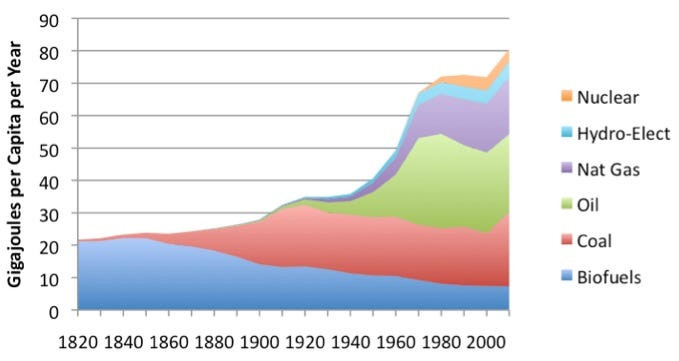
\includegraphics[scale=0.35]{media/world_per_capita_energy.jpeg}
  \caption{
      Consommation d'énergie par personne\newline
      \tiny{Source:\newline
        \url{https://www.businessinsider.com/a-worrying-look-at-world-energy-consumption-since-1820-2012-3?IR=T}
      }
  }
  \label{fig:capita_energy}
\end{SCfigure}

Cette augmentation de consommation d'énergie par habitant 
s'ajoute a une augmentation massive de la population sur Terre.

\begin{SCfigure}[][h]
  \centering
  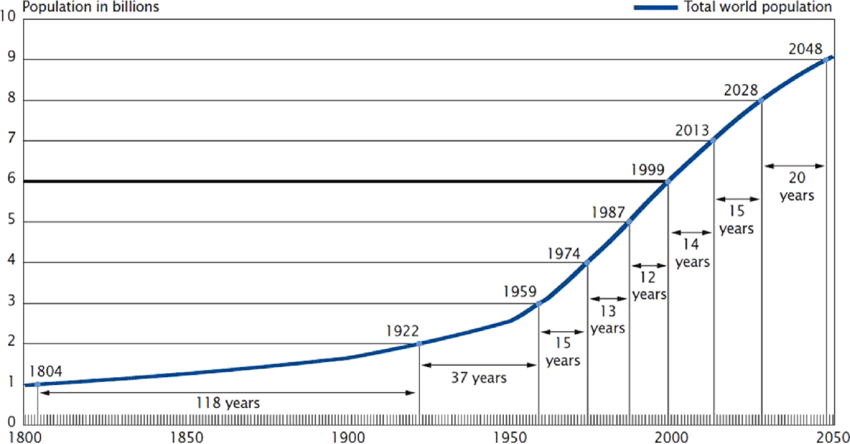
\includegraphics[scale=0.35]{media/WorldPopulation.png}
  \caption{
      Population sur Terre\newline
      \tiny{Source:\newline
        \url{https://www.researchgate.net/figure/World-Population-1800-2050-6_fig1_321996838}
      }
  }
  \label{fig:capita_energy}
\end{SCfigure}

\section{Guerre de l'énergie}

Le concept de la guerre est toujours le même depuis des millénaires, prendre posséssion des
ressources de l'autre pour son propre avantage.

Nous pouvons citer quelque types de guerre qui mettent a profit la faiblesse des uns
pour enrichir les plus fort :

\begin{itemize}
  \item la délimitation des territoires % ont toujours été source de conflits entraînant
  % des guerres se traduisant par la perte de vies humaines.
  \item les consommables comme les ressources agricole ou épices
  \item les connaissances et technologies
  \item les sources énergétiques
\end{itemize}

La guerre est bien plus rare de nos jours, de nombreuses instances telle que l'ONU ou bien les
contrats commerciaux ont rendu les conflits directs moins rentable.

Aujourd'hui, les foyers de tensions n’ont pourtant pas disparu tout autant,
ce sont essentiellement les mêmes depuis trente ans et ont tous un point communs,
ils possèdent du pétrole en sous-sol.

Le golfe Persique est au bord de la guerre civile alors qu'il représente 67\%
de la production pétrolier mondiale, ainsi que 40\% des réserves mondiales de gaz.

Cependant, le fait que ces guerres concernent l'énergie pétrolière les rendent éphémères,
en effet les réserves ne font que baisser sans se renouveler, ce qui déplacera les
guerres vers une autre source et probablement une autre localisation géographique.

Quelques ressources commencent a cristalliser des tensions, ce qui peut nuire à la paix
dans ces régions.

Au maghreb les ressources en eau sont contesté entre l'Algérie, la Tunisie et la Libye, ces
trois pays clament la possession des eaux de la nappe phréatique s'étalant sous leurs
territoires.

\begin{SCfigure}[][h]
  \centering
  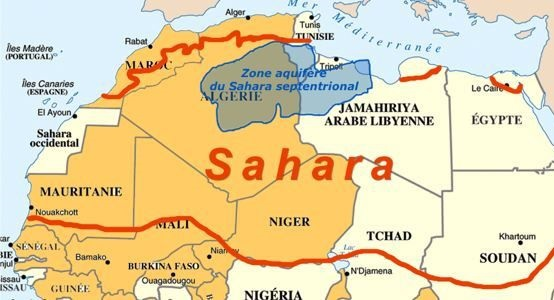
\includegraphics[scale=0.35]{media/zone_aquifere_sahara.jpg}
  \caption{
    Nappe phréatique au maghreb\newline
      \tiny{Source:\newline
        \url{https://i1.wp.com/www.webdo.tn/wp-content/uploads/2014/03/Carte-photo-canalblog.jpg}
      }
  }
  \label{fig:zone_aquifere_sahara}
\end{SCfigure}

Autre ressource, autre cause de conflit, les terres rares sont inégalement réparties
sur terre avec la Chine qui possèdent près de 60\% des réserves mondiales.

\begin{SCfigure}[][h]
  \centering
  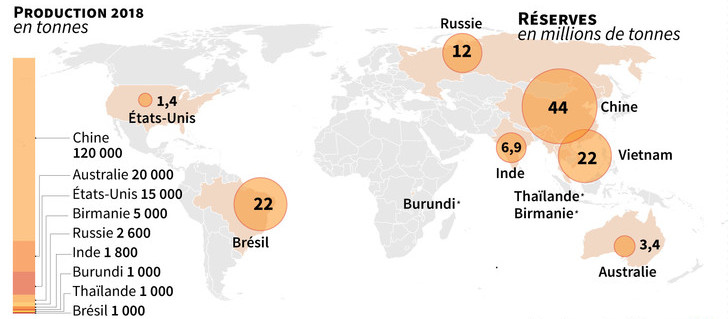
\includegraphics[scale=0.5]{media/terres_rares.jpg}
  \caption{
    Production et réserves de métaux rares\newline
      \tiny{Source:\newline
        \url{https://img.aws.la-croix.com/2019/05/29/1301025438/Production-reserves-metaux-rares_1_728_388.jpg}
      }
  }
  \label{fig:terre_rare}
\end{SCfigure}

\section{Amélioration des performances informatique}

La technologie est en constante progression depuis toujours.
L'augmentation de cycle d'horloge, de stockage et de vitesse de traitement de donnée
ont changer la manière dont l'Homme communique avec la machine.

Aujourd'hui l'humain peut parler en langage naturel à des assistant personnel pour combler ses
besoin du quotidien. 
Ces besoin nouveaux s'inscrivent dans une dynamique datant de l'ère industriel qui veux que
la population améliore sa qualité de vie quotidienne.

Grâce à ces performances, un français moyen vie une vie plus confortable qu'un roi 
du moyen-age.

Le futur vois une réductions de cette augmentation de performance, mais de meilleurs collaboration
entre elles, le scaling deviens verticale et non horizontale.

% Image montrant l'augmentation de performance


